\documentclass[a4paper,12pt]{article}
\usepackage{CJKutf8}
\usepackage{indentfirst}
\usepackage{graphicx}
\usepackage{amsmath}
\usepackage{longtable}
\usepackage{fancyhdr}
\usepackage{multirow}
\usepackage{setspace}
\usepackage{booktabs}
\usepackage{daytime}
\usepackage{cite}

\renewcommand{\today}{\number\year 年 \number\month 月 \number\day 日}

\pagestyle{fancy}
\setlength{\textwidth}{159.2mm}
\setlength{\oddsidemargin}{0pt}
\setlength{\voffset}{-10mm}
\setlength{\headwidth}{159.2mm}
\setlength{\textheight}{235mm}
\fancyhf{}
\lhead{\begin{CJK*}{UTF8}{gkai}CVDL大作业\end{CJK*}}
\rhead{\thepage}

\begin{document}
\begin{CJK*}{UTF8}{gbsn}

\title{\textbf{CVDL大作业\\期末报告}}
\author{葛博文\;1500019707\\周清逸\;1500012930}
\date{\today}
\maketitle

\begin{spacing}{1.2}

    \section{任务动机}
    在一次寒假调研时,我们意外地发现,尽管地方政府对农业用地早已有了诸多保护政策,农业用地违法挪用建造商品房以谋取私利的情况依然广大范围内存在。这种行为对我国的农业生产工作产生了极大的危害,必须严加监管。而这现象屡禁不止的原因之一,是高层政府对于农业用地的实际监管困难。因此我们希望做一个程序来试图识别农业用地的实际使用情况。


    \section{任务分析}
    如何从遥感卫星图片判断一块土地是否为农业用地是一个比较泛泛的概念。考虑到很多土地挪用是为了商品房建造,同时房屋的数据集也5比较容易得到,因此我们可以将这个土地使用方式识别的任务转化为在一片地图上寻找房屋的任务。我们从“一个网站”上得到了有关房屋的数据集\cite{maggiori2017dataset}。初步分析数据集我们可以猜想这个任务的主要难点在于:
    \begin{itemize}
        \item 房子数量多而分布密集,单个房子却很小,会对网络产生压力。
        \item 由于光照问题,房屋和树木遮挡,会相应地产生阴影投射到房子上,对于网络的识别增加了困难。
        \item 不同数据集之间差别很大,而且不均匀。例如有些城市沿海,就会有少量的水面和船等景象,然而这些数量很小,不能在网络中充分训练。
        \item 房屋和船、大卡车等物品天生很像。
        \item 在这些数据集上有关绿地的部分主要为树木和草地,而作为我们最终目标的中国地区作为测试的图片中,却主要为农田,这样的数据集变化可能会导致很糟糕的效果。
    \end{itemize}



    \section{图片预处理}
    我们使用的数据集的特点如下:
    \begin{itemize}
        \item 包含覆盖了$810km^2$(其中$405km^2$用于训练集,$405km^2$用作测试集)。
        \item 是空间分辨率为0.3m的正交矫正彩色图像。
        \item 标签是二分类分割:是房子和不是房子。
        \item 这些图像涵盖了不同的城市住区,从人口稠密地区(例如旧金山金融街)到高山城镇(例如奥地利蒂罗尔的利恩茨)。
    \end{itemize}
    我们先将原先大小为$5000\times5000$的图片补成$5120\times5120$($padding=60$)的大小。然后将按照步长160($stride=160$)其顺序切成961张$320\times320$的小图。\\
    我们随后对图片做的数据增强如下:
    \begin{itemize}
        \item 将图片旋转一个随机的角度
        \item 将图片随机水平和数值翻转
        \item 将图片加入高斯噪声
        \item 随机调整图片的亮度、对比度、饱和度和色调
    \end{itemize}
    同时也对标签做相同的旋转和翻转的变换。\\
    我们这样做的原因是主要考虑到对于美国城市而言,房子的方向大多是极其统一的,而卫星的拍照方向固定,将造成训练集中大量的房屋方向相同,这样将使得网络的训练数据过于局限。在此考虑下,我们决定引入图片的旋转和翻转,这样可以引入训练集的随机性,用于增强网络的范性。同时,由于不同城市不同国家的房屋整体色调也有所不同,于是我们希望淡化网络对特定颜色的认知,而主要提取形状特征,这样调整图片的色调就是必要的。同时为了增强网络的鲁棒性,我们也对输入训练数据加入了高斯噪声。




    \section{网络结构}
    任务本身属于语义分割。用深度学习进行语义分割的方法多种多样,在本次任务中我们决定采用U-Net,如图所示。
    \begin{figure} [!]
    \centering
    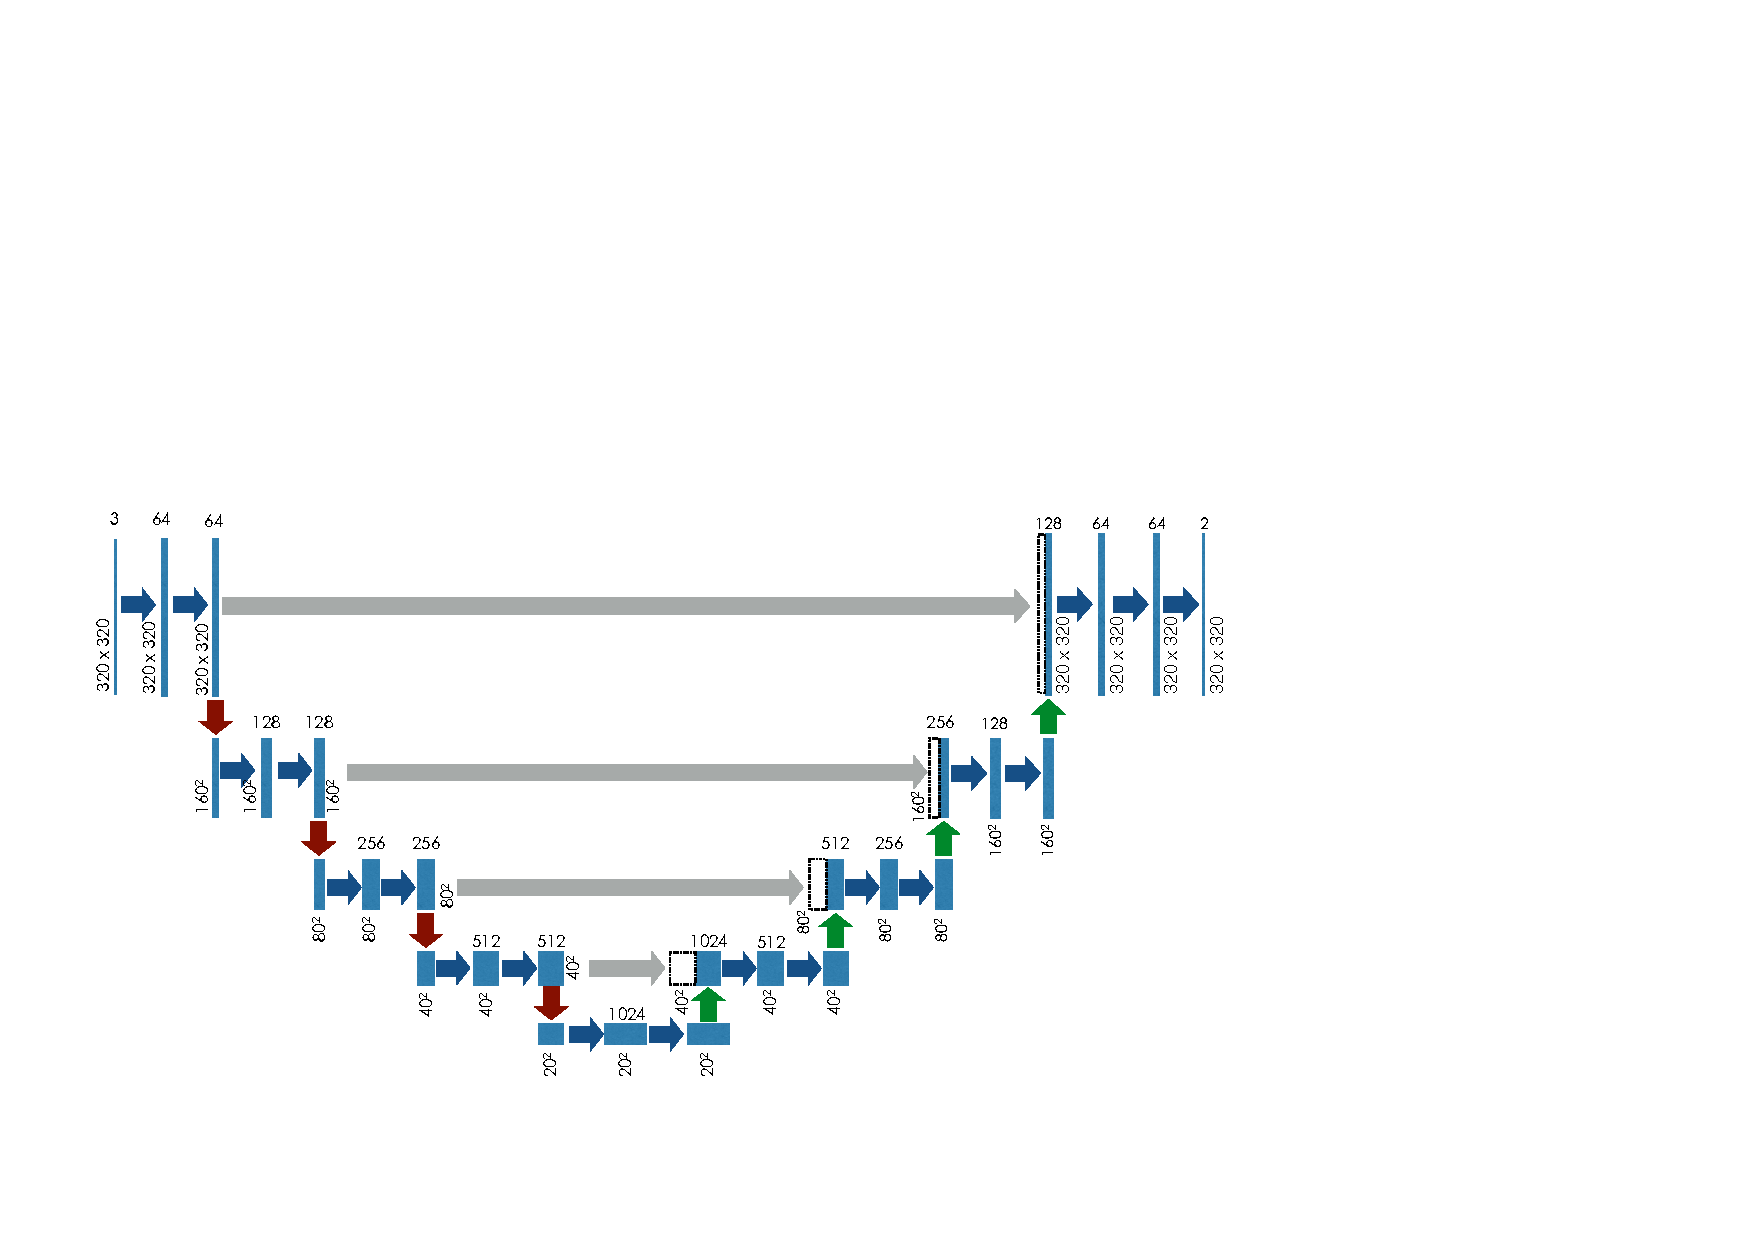
\includegraphics[width=14.0cm]{U_Net.pdf}
    \caption{A schematic illustration of U-Net's structure.}
    \label{fig:Fig 1}
    \end{figure}
    采用U-Net的原因主要是由于结构清晰:属于典型的Encoder-Decoder架构,专门为分割任务设计,考虑到单纯的Encoder-Decoder型网络会丢失图片细节,加入了short-cut,通过将不同尺度的信息进行拼接的方式,缓解了细节的丢失。
    
    最初使用一个U-Net进行测试的效果并不是很理想,于是我们尝试将两个U-Net拼接在一起,希望通过增加模型的深度,取得更好的效果。然而在训练时,拼接的模型很快就出现了过拟合现象,在验证集上的loss无法很好地收敛,泛化性能很差,因此最终我们没有采用这一模型。
    
    \subsection{Loss函数}
    如果简单地把分割任务看作一个二分类,在网络的最后一层使用Softmax激励函数,得到每个像素分属于两类(建筑/非建筑)的概率,那么可以直接用交叉熵作为Loss函数。从代码train.py中可以看到,pyTorch中对于分割问题的Loss,使用的是Nllloss()函数,此时网络最后一层是logsoftmax,但本质是相同的。
    
    对于二分类问题,交叉熵的表达式可以写作:
    \begin{equation}
    L = -\frac{1}{N}\sum[y_{i}\ln(p_{i}) + (1-y_{i})\ln(1-p_{i})].
    \end{equation}
    在模型V1.0中,我们直接使用交叉熵作为Loss函数,效果比较差,存在很多大量False negative,很多建筑物无法判断出来。False negative较多的主要原因是正负样本不均衡,因此在此后的模型中,我们决定调整交叉熵表达式中两项的权重。根据参考文献\cite{},最直接的解决方法是计算正负两类所占的比例$\alpha_{0}$和$\alpha_{1}$(自然满足$\alpha_{0}+\alpha_{1}=1$),然后将两项分别乘上对应的系数:
    \begin{equation}
    L = -\frac{1}{N}\sum[\alpha_{0}y_{i}\ln(p_{i}) + \alpha_{1} (1-y_{i})\ln(1-p_{i})].
    \end{equation}
    经过统计,在数据集中,建筑物对应的像素所占比例约为$15\%-20\%$,因此在模型V1.2中,采用比例$\alpha_{1}=0.2$。这样,如果对于某个像素满足$y_{i}=1$,但预测${p_{i}}$明显小于1,乘以$\alpha_{0}$相当于对此类情形施加惩罚,从而一定程度上解决正负样本不均的问题。
    
    一般而言,针对语义分割任务,一个重要的评价标准是IoU。实际上IoU比单纯计算准确率更加合理(对于建筑物只占$15\%$的情形,预测全0便可以达到$85\%$的准确率)。对于一个类别而言,记预测的mask为$X$,实际的mask为$Y$,IoU的定义为:
    \begin{equation}
    \rm{IoU} = \frac{\left |{X}\bigcap{Y}\right |}{\left |{X}\bigcup{Y}\right |}.
    \end{equation}
    
    经过查阅资料\cite{},针对IoU可以设计更为合理的Loss。根据$Y$和预测的$X$定义Dice系数:
    \begin{equation}
    \rm{DSC} = \frac{2 \left |{X}\bigcap{Y}\right |}{\left |X \right |+ \left |Y\right |}.
    \end{equation}
    直观来说,Dice系数形式上比较接近IoU。为了达到最大化IoU的目的,可以尝试将Dice系数加入Loss函数。包含$X$的Dice系数是不可导的,因此记$P$为预测的概率(不转化为0/1标签),定义非负的$\rm{DSC}_{diff}$为:
    \begin{equation}
    \rm{{DSC}_{diff}} = \frac{2\sum y_{i}p_{i}}{\sum p_{i} + \sum{y_{i}}}.
    \end{equation}
    当完美预测时(所有标签为1的像素,预测为建筑的概率均为$1$),$\rm{DSC}_{diff}$达到1。在Kaggle比赛中,有人采用$1-\rm{DSC}_{diff}$作为Loss函数中的一项。在本次实验中,为了对IoU较小的预测施加更大的惩罚力度,我们将$-\ln(\rm{DSC}_{diff})$加入Loss函数中(在$\rm{DSC}_{diff}$接近1的时候二者相近)。对于模型V1.4,我们采用如下形式的Loss函数进行训练:
    \begin{equation}
    L = -\frac{1}{N}\sum[(1-\alpha_{1})y_{i}\ln(p_{i}) + \alpha_{1} (1-y_{i})\ln(1-p_{i})] - \beta \ln(\rm{DSC}_{diff}).
    \end{equation}
    
    我们在报告后面会对各个不同模型进行测试,测试条件和结果汇总在表格当中。



    
    \bibliography{reference}
    
\end{spacing}
\end{CJK*}
\end{document}